\chapter{Robustness Analysis}

\label{Chapter-Robustness-Analysis}

In this chapter, AlexNet's \cite{ImageNet-classification-with-deep-convolutional-neural-networks} structure is analyzed and modeled using MATLAB \cite{MATLAB-Official-site} and C/C++, evaluating the results using PyTorch \cite{PyTorch-Official-site}. As a starting point, the prebuilt and pre-trained AlexNet model provided by PyTorch was used. For a better understanding of the underlining algorithms, a C/C++ library was created to replicate PyTorch's functionality, from image and parameter importing and formatting, to every CNN layer type needed for the network's inference.

Moreover, a Sensitivity Analysis was performed to explore hardware implementation opportunities. Furthermore, various quantization techniques and algorithmic optimizations have been studied and tested to reduce memory footprint and better utilize hardware resources. Lastly, several implementation techniques and tools on the same functionality have been studied to minimize hardware resources and latency.

\section{PyTorch and C/C++ implementations}
Since PyTorch is a high abstraction framework, the recreation of its functionality to a lower abstraction level language, like C/C++, is a necessity for a complete understanding of the neural network's operation mechanism. Hence, after creating a C/C++ library capable of implementing most CNNs, it was evaluated for its correctness using PyTorch as a baseline. Its evaluation was conducted by implementing AlexNet, as an example network, using both PyTorch and the C/C++ library, and then running the network's inference on both implementations for 2500 input images. Afterward, the results, taken from the last FC layer of both implementations, were compared to create an error rate for each input. The library is designed in a way that it can use any data type for weights and activations to enable further experimentations. This evaluation experiment was conducted two times, one for using double-precision and another for using single-precision floating-point data type (IEEE standard). The error rate of both experiments was almost zero, with some minor inconsistencies between the floating-point representations of C/C++ and Python. Thus, both implementations' classifications were fully matched, and the library can be characterized as correct.

\subsection{Algorithms}
The main building blocks of a typical 2-D CNN is presented below.

\subsubsection{Convolution}
Algorithm \ref{alg:Convolution-Layer} performs a 2-D Convolution on 3-D array inputs, like images. The \textit{input} is characterized by its height, its width, and its number of channels. In other words, the number of its parallel matrices; for an RGB image, there are three channels, one for every color. The \textit{kernelSize}, \textit{stride} and \textit{padding} are the hyper-parameters of convolution layers, and because they differ for every layer and network, they have to be included in the procedure's parameters. Last but not least, \textit{weights} and \textit{bias} are the networks parameters. This algorithm outputs a 3-D array with the convolution's results.

\begin{algorithm}[H]
	\caption{Convolution Layer}\label{alg:Convolution-Layer}
	\begin{algorithmic}[1]
		\Procedure{Convolution Layer}{input, kernelSize, stride, padding, weights, bias}
			\State $hOut \gets (input.height +2 * padding - kernelSize) / stride + 1$
			\State $wOut \gets (input.width +2 * padding - kernelSize) / stride + 1$

			\For{i:=1 \textbf{to} input.channels}
				\For{j:=1 \textbf{to} input.height + 2 * padding}
					\For{k:=1 \textbf{to} input.width + 2 * padding}
						\If{j < padding || k < padding || j > image.height || k > image.height}
							\State $arr(i, j, k) \gets 0$
						\Else{}
							\State $arr(i, j, k) \gets input(i, j - padding, k - padding)$
						\EndIf
					\EndFor
				\EndFor
			\EndFor

			\For{oc:=1 \textbf{to} size(weights, 1)} \Comment{\#Output channels}
				\For{oh:=1 \textbf{to} hOut}
					\State $imgStartH \gets oh * stride$
					\State $imgEndH \gets imgStartH + kernelSize$

					\For{ow:=1 \textbf{to} wOut}
						\State $imgStartW \gets ow * stride$
						\State $imgEndW \gets imgStartW + kernelSize$

						\State $pixel \gets 0$
						\For{ic:=1 \textbf{to} input.channels}
							\For{i:=1 \textbf{to} kernelSize}
								\For{j:=1 \textbf{to} kernelSize}
									\State $pixel \gets pixel + arr(ic, i + imgStartH, j + imgStartW) * weights(oc, ic, i, j)$
								\EndFor
							\EndFor
						\EndFor

						\State $output(oc, oh, ow) \gets pixel + bias(oc)$
					\EndFor
				\EndFor
			\EndFor
			\State \textbf{return} $output$
		\EndProcedure
	\end{algorithmic}
\end{algorithm}

Algorithm \ref{alg:Convolution-Layer-with-ReLU} is a slightly more optimized version of algorithm \ref{alg:Convolution-Layer}. Since padding creates areas of the input that are zeroed out, convolution on those areas results in zero. Therefore, the for-loops' indices are carefully calculated to avoid iterations on the padded areas. Furthermore, the creation of the "padded" input is also omitted.

Moreover, a small optimization is injecting the ReLU activation function into this algorithm. Provided that ReLU is used almost after every convolution layer, this optimization avoids rereading the whole input from memory to make a simple decision. The procedure's \textit{doRelu} parameter configures if the ReLU activation is used.

\begin{algorithm}[H]
	\caption{Convolution Layer with ReLU}\label{alg:Convolution-Layer-with-ReLU}
	\begin{algorithmic}[1]
		\Procedure{Convolution Layer with ReLU}{input, kernelSize, stride, padding, weights, bias, doRelu}
			\State $hOut \gets (input.height +2 * padding - kernelSize) / stride + 1$
			\State $wOut \gets (input.width +2 * padding - kernelSize) / stride + 1$

			\For{oc:=1 \textbf{to} size(weights, 1)} \Comment{\#Output channels}
				\For{oh:=1 \textbf{to} hOut}

					\State $imgStartH \gets oh * stride - padding$

					\State $iStart \gets imgStartH < 0 ? padding : 0$

					\If{$imgStartH + kernelSize \geq input.height$}
						\State $iEnd \gets kernelSize - (imgStartH + kernelSize - input.height)$
					\Else{}
						\State $iEnd \gets kernelSize$
					\EndIf

					\For{ow:=1 \textbf{to} wOut}
						\State $imgStartW \gets ow * stride - padding$

						\State $jStart \gets imgStartW < 0 ? padding : 0$

						\If{$imgStartW + kernelSize \geq input.height$}
							\State $jEnd \gets kernelSize - (imgStartW + kernelSize - input.height)$
						\Else{}
							\State $jEnd \gets kernelSize$
						\EndIf

						\State $pixel \gets bias(oc)$

						\For{ic:=1 \textbf{to} input.channels}
							\For{i:=iStart \textbf{to} iEnd}
								\For{j:=jStart \textbf{to} jEnd}
									\State $pixel \gets pixel + input(ic, i + imgStartH, j + imgStartW) * weights(oc, ic, i, j)$
								\EndFor
							\EndFor
						\EndFor

						\State $output(oc, oh, ow) \gets doRelu \&\& pixel < 0 ? 0 : pixel$
					\EndFor
				\EndFor
			\EndFor
			\State \textbf{return} $output$
		\EndProcedure
	\end{algorithmic}
\end{algorithm}

\subsubsection{MaxPool}
Algorithm \ref{alg:MaxPool-Layer} performs a 2-D max-pooling operation on 3-D array inputs. Likewise to the convolution algorithm's \textit{input}, it is characterized by its height, width, and channel number. Also the \textit{kernelSize} and \textit{stride} hyper-parameters are present, in contrast to padding, which is not used, so it is omitted. This algorithm outputs a 3-D array with the max-pooling operation's results.

\begin{algorithm}[H]
	\caption{MaxPool Layer}\label{alg:MaxPool-Layer}
	\begin{algorithmic}[1]
		\Procedure{MaxPool Layer}{input, kernelSize, stride}
			\State $hOut \gets (input.height - kernelSize) / stride + 1$
			\State $wOut \gets (input.width - kernelSize) / stride + 1$
			\For{i:=1 \textbf{to} input.channels}
				\For{j:=1 \textbf{to} hOut}
					\For{k:=1 \textbf{to} wOut}
						\State $max \gets -\infinity$
						\For{l:=1 \textbf{to} kernelSize}
							\For{m:=1 \textbf{to} kernelSize}
								\State $curHeight \gets j * stride + l$
								\State $curWidth \gets k * stride + l$
								\State $curPixel \gets input(i, curHeight, curWidth)$
								\If{max < curPixel}
									\State $max \gets curPixel$
								\EndIf
							\EndFor
						\EndFor
						\State $output(i, j, k) \gets max$
					\EndFor
				\EndFor
			\EndFor
			\State \textbf{return} $output$
		\EndProcedure
	\end{algorithmic}
\end{algorithm}

\subsubsection{Fully-Connected}
Algorithm \ref{alg:Fully-Connected-Layer} performs a matrix multiplication on the \textit{input} and \textit{weights}. The \textit{input} is a vector, either coming from the previous FC layer's output or the flattening of the previous convolution or max-pooling layer's results. After the matrix multiplication a \textit{bias} is accumulated. This algorithm outputs a vector with the results of the matrix multiplication.

\begin{algorithm}[H]
	\caption{Fully-Connected Layer}\label{alg:Fully-Connected-Layer}
	\begin{algorithmic}[1]
		\Procedure{Fully-Connected Layer}{input, weights, bias}
			\State $inputSize \gets size(input)$
			\State $outputSize \gets size(weights, 1)$
			\For{i:=1 \textbf{to} outputSize}
				\State $output(i)\gets bias(i)$
				\For{j:=1 \textbf{to} inputSize}
					\State $output(i)\gets output(i) + input(j) * weights(i, j)$
				\EndFor
				\If{doRelu \&\& output(i) < 0}
					\State $output(i) \gets 0$
				\EndIf
			\EndFor
			\State \textbf{return} $output$
		\EndProcedure
	\end{algorithmic}
\end{algorithm}

Algorithm \ref{alg:Fully-Connected-Layer-with-ReLU} is a slightly more optimized version of algorithm \ref{alg:Fully-Connected-Layer}. Likewise to the convolution algorithm \ref{alg:Convolution-Layer-with-ReLU}, the ReLU activation is injected and can be configured through the \textit{doReLU} parameter.

\begin{algorithm}[H]
	\caption{Fully-Connected Layer with ReLU}\label{alg:Fully-Connected-Layer-with-ReLU}
	\begin{algorithmic}[1]
		\Procedure{Fully-Connected Layer with ReLU}{input, weights, bias, doReLU}
			\State $inputSize \gets size(input)$
			\State $outputSize \gets size(weights, 1)$
			\For{i:=1 \textbf{to} outputSize}
				\State $output(i)\gets bias(i)$
				\For{j:=1 \textbf{to} inputSize}
					\State $output(i)\gets output(i) + input(j) * weights(i, j)$
				\EndFor
				\If{doRelu \&\& output(i) < 0}
					\State $output(i) \gets 0$
				\EndIf
			\EndFor
			\State \textbf{return} $output$
		\EndProcedure
	\end{algorithmic}
\end{algorithm}

\subsubsection{ReLU}
While ReLU activation function is already injected to the convolution \ref{alg:Convolution-Layer-with-ReLU} and FC \ref{alg:Fully-Connected-Layer-with-ReLU} algorithms, its algorithms are shown below for completeness. Algorithm \ref{alg:ReLU1D)} performs the ReLU activation on vector inputs, suitable for use after FC layers. Algorithm \ref{alg:ReLU3D)} performs the ReLU activation on 3-D data inputs, suitable for use after convolution and max pooling layers.

\begin{algorithm}[H]
	\caption{ReLU (1-D)}\label{alg:ReLU1D)}
	\begin{algorithmic}[1]
		\Procedure{ReLU (1-D)}{input}
			\For{i:=1 \textbf{to} size(input)}
				\If{input(i) > 0}
					\State $output(i) \gets input(i)$
				\Else{}
					\State $output(i) \gets 0$
				\EndIf
			\EndFor
			\State \textbf{return} $output$
		\EndProcedure
	\end{algorithmic}
\end{algorithm}

\begin{algorithm}[H]
	\caption{ReLU (3-D)}\label{alg:ReLU3D)}
	\begin{algorithmic}[1]
		\Procedure{ReLU (3-D)}{input}
			\For{i:=1 \textbf{to} size(input, 1)}
				\For{j:=1 \textbf{to} size(input, 2)}
					\For{k:=1 \textbf{to} size(input, 3)}
						\If{input(i, j, k) > 0}
							\State $output(i, j, k) \gets input(i, j, k)$
						\Else{}
							\State $output(i, j, k) \gets 0$
						\EndIf
					\EndFor
				\EndFor
			\EndFor
			\State \textbf{return} $output$
		\EndProcedure
	\end{algorithmic}
\end{algorithm}

\subsubsection{SoftMax}
Algorithm \ref{alg:SoftMax} performs a SoftMax activation function on vector inputs. This operation is applied after the last FC layer and outputs the probability distribution of each target class.

\begin{algorithm}[H]
	\caption{SoftMax}\label{alg:SoftMax}
	\begin{algorithmic}[1]
		\Procedure{SoftMax}{$input$}
			\State $sum \gets 0$

			\For{i:=1 \textbf{to} size(input)}
				\State $sum \gets sum + e^{input(i)}$
			\EndFor

			\For{i:=1 \textbf{to} size(input)}
				\State $output \gets e^{input(i)} / sum$
			\EndFor

			\State \textbf{return} $output$
		\EndProcedure
	\end{algorithmic}
\end{algorithm}

\section{Data Types}
As mentioned in the Related Work section, memory bandwidth needs can become a severe bottleneck to applications like neural networks on FPGAs and ASICs. Consequently, the investigation of the most suitable data type is a necessity. However, decreasing the bit-width does come with its costs, classification accuracy. This creates a tradeoff between network classification accuracy and inference speed. In general, lowering the bit-width increases performance, but decreases accuracy. The cost of each bit-width lowering is different for every application, so a specific investigation has to be done.

% Todo: Fix text on data types
Using AlexNet as a reference, two different data types have been used: single, and half-precision floating-point (IEEE standard). This experiment's baseline uses a single-precision floating-point, as it has full data precision given from the pre-trained model. After inferencing 2500 images using both data types, each image classification Top-1 result was compared to the baseline's result. The Top-1 error rate for each data type is presented in table \ref{tab:floats-error-rates}.

% Todo: fill table with correct data
\begin{table}[H]
	\caption{Floating-point precision Top-1 error rates}
	\label{tab:floats-error-rates}
	\centering
	\begin{tabular}{l l l}
		\toprule
		\textbf{Data type} & \textbf{Top-1 Error rate(\%)} & \textbf{Running time (ms)} \\
		\midrule
			Single-precision floating-point	& 0			& 0 \\
			Half-precision floating-point 	& 0.0036 	& 0 \\
			8-bit Fixed point & 0 & 0 \\
			10-bit Fixed point & 0 & 0 \\
			12-bit Fixed point & 0 & 0 \\
			16-bit Fixed point & 0 & 0 \\
			32-bit Fixed point & 0 & 0 \\
			64-bit Fixed point & 0 & 0 \\
		\bottomrule\\
	\end{tabular}
\end{table}

% Todo: Fix text on data types
It is worth noting that a MATLAB implementation of the network had to be used in this investigation, due to the fact that, at the time of writing, neither PyTorch nor C/C++ support half-precision floating-point arithmetic. Unfortunately, MATLAB inference was really slow compared to PyTorch, and even slower when using half-precision. The half-precision floating-point slowdown was caused because there is no hardware acceleration on the test CPU (Intel i7 4710MQ) for such data type.

\section{Memory Footprint}

\begin{table}[H]
	\caption{AlexNet Parameters Memory Footprint}
	\label{tab:AlexNet-Parameters-Memory-Footprint}
	\centering
	\begin{tabular}{llll}
		\toprule
		\textbf{Layer} & \textbf{\#Parameters} & \textbf{Footprint} & \textbf{Memory (\%)}  \\
		\midrule
			Conv1 & $64 * 3 * 11 * 11 = 23232$ & 92.92KB & 0.04 \\
			Conv2 & $192 * 64 * 5 * 5 = 307200$ & 1.22MB & 0.5 \\
			Conv3 & $384 * 192 * 3 * 3 = 663552$ & 2.65MB & 1.09 \\
			Conv4 & $256 * 384 * 3 * 3 = 884736$ & 3.53MB & 1.45 \\
			Conv5 & $256 * 256 * 3 * 3 = 589824$ & 2.35MB & 0.97 \\
			FC1 & $9216 * 4096 = 37748736$ & 150.99MB & 61.79 \\
			FC2 & $4096 * 4096 = 16777216$ & 67.10MB & 27.46 \\
			FC3 & $4096 * 1000 = 4096000$ & 16.38MB & 6.70 \\
		\midrule
			\textbf{Total} & 61090496 & 244.36MB & 100 \\
		\bottomrule\\
	\end{tabular}
\end{table}

\begin{table}[H]
	\caption{AlexNet Data Stages Memory Footprint}
	\label{tab:AlexNet-Data-Stages-Memory-Footprint}
	\centering
	\begin{tabular}{llll}
		\toprule
		\textbf{Layer} & \textbf{\#Data} & \textbf{Footprint} & \textbf{Memory (\%)}  \\
		\midrule
			Image & $3 * 224 * 224 = 150528$ & 150.52KB & 6.07 \\
			Conv1 & $64 * 55 * 55 = 193600$ & 774.40KB & 31.22 \\
			MaxPool1 & $64 * 27 * 27 = 46656$ & 186.62KB & 7.52 \\
			Conv2 & $192 * 27 * 27 = 139968$ & 559.87KB & 22.57 \\
			MaxPool2 & $192 * 13 * 13 = 32448$ & 129.79KB & 5.23 \\
			Conv3 & $384 * 13 * 13 = 64896$ & 259.58KB & 10.46 \\
			Conv4 & $256 * 13 * 13 = 43264$ & 173.05KB & 6.98 \\
			Conv5 & $256 * 13 * 13 = 43264$ & 173.05KB & 6.98 \\
			MaxPool3 & $9216$ & 36.86KB & 1.49 \\
			FC1 & $4096$ & 16.38KB & 0.66 \\
			FC2 & $4096$ & 16.38KB & 0.66 \\
			FC3 & $1000$ & 4KB & 0.16 \\
		\midrule
			\textbf{Total} & 682856 & 2.48MB & 100 \\
		\bottomrule\\
	\end{tabular}
\end{table}

\section{Weight Distribution}



\begin{figure} [H]
	\centering
	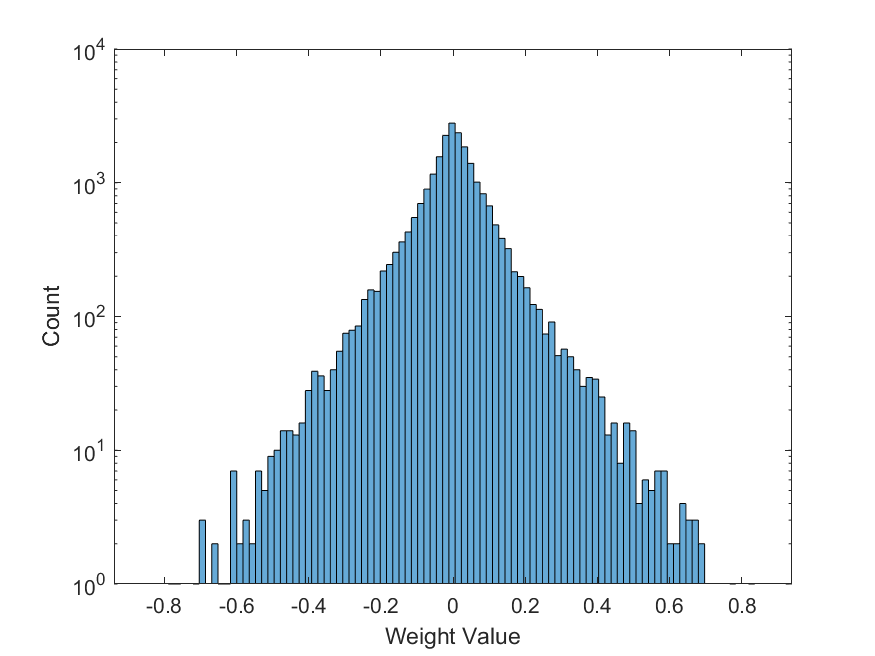
\includegraphics[scale=0.9]{Images/Weights/weight-distribution-conv1.png}
	\decoRule
	\caption[Weights distribution of 1st Convolution layer]{Weights distribution of 1st Convolution layer}
	\label{fig:weight-distribution-conv1}
\end{figure}

\begin{figure} [H]
	\centering
	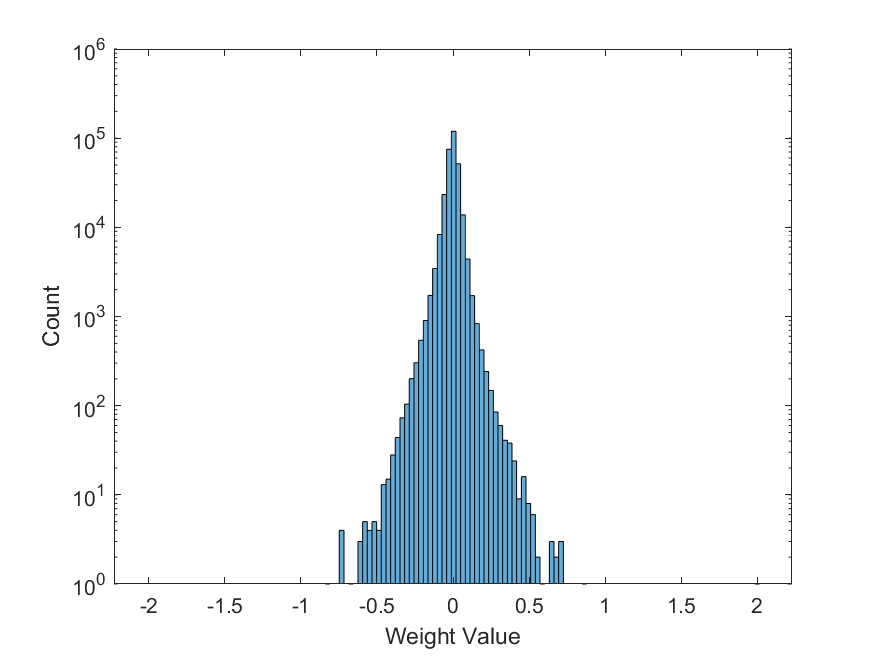
\includegraphics[scale=0.9]{Images/Weights/weight-distribution-conv2.png}
	\decoRule
	\caption[Weights distribution of 2nd Convolution layer]{Weights distribution of 2nd Convolution layer}
	\label{fig:weight-distribution-conv2}
\end{figure}

\begin{figure} [H]
	\centering
	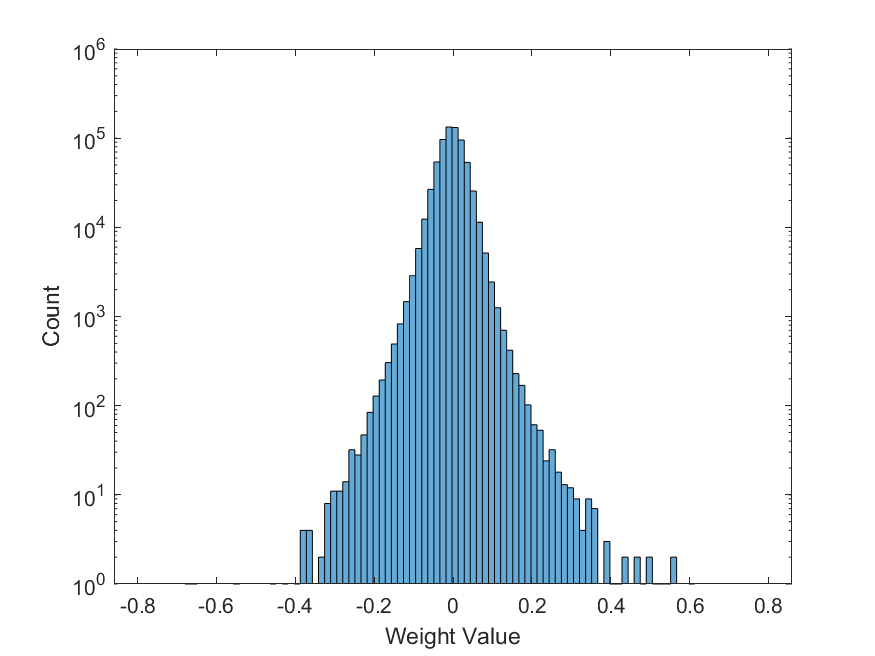
\includegraphics[scale=0.9]{Images/Weights/weight-distribution-conv3.png}
	\decoRule
	\caption[Weights distribution of 3rd Convolution layer]{Weights distribution of 3rd Convolution layer}
	\label{fig:weight-distribution-conv3}
\end{figure}

\begin{figure} [H]
	\centering
	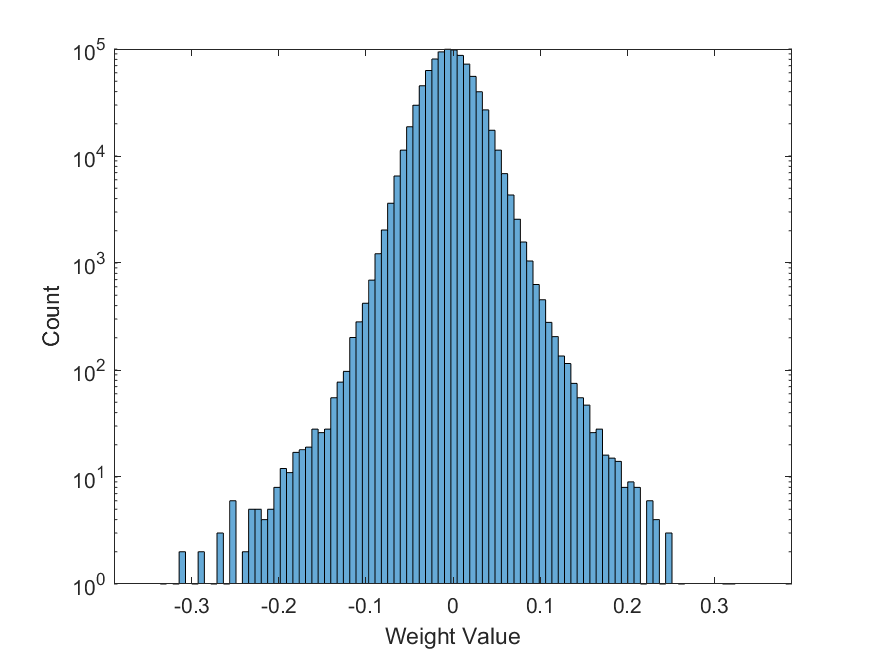
\includegraphics[scale=0.9]{Images/Weights/weight-distribution-conv4.png}
	\decoRule
	\caption[Weights distribution of 4th Convolution layer]{Weights distribution of 4th Convolution layer}
	\label{fig:weight-distribution-conv4}
\end{figure}

\begin{figure} [H]
	\centering
	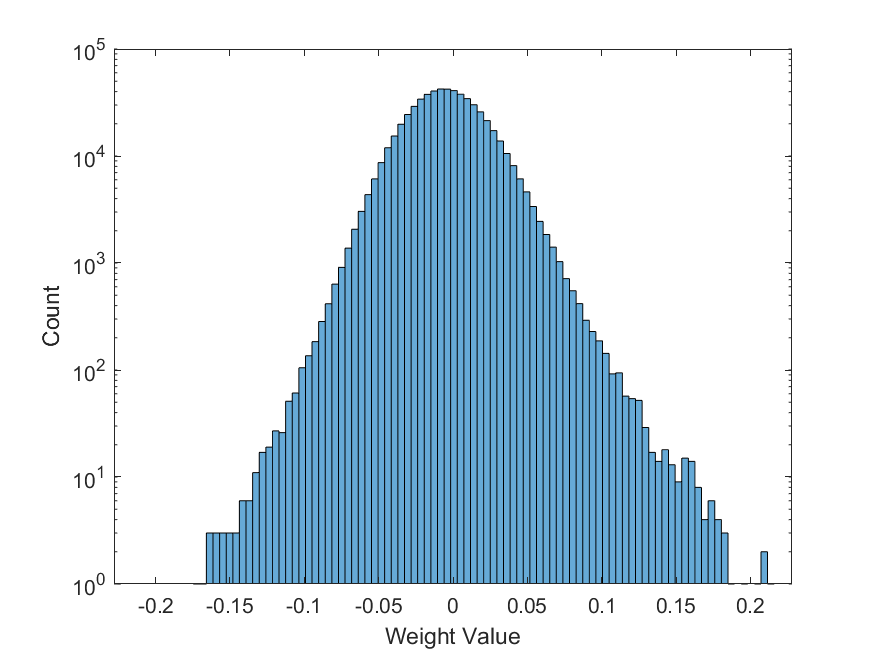
\includegraphics[scale=0.9]{Images/Weights/weight-distribution-conv5.png}
	\decoRule
	\caption[Weights distribution of 5th Convolution layer]{Weights distribution of 5th Convolution layer}
	\label{fig:weight-distribution-conv5}
\end{figure}

\begin{figure} [H]
	\centering
	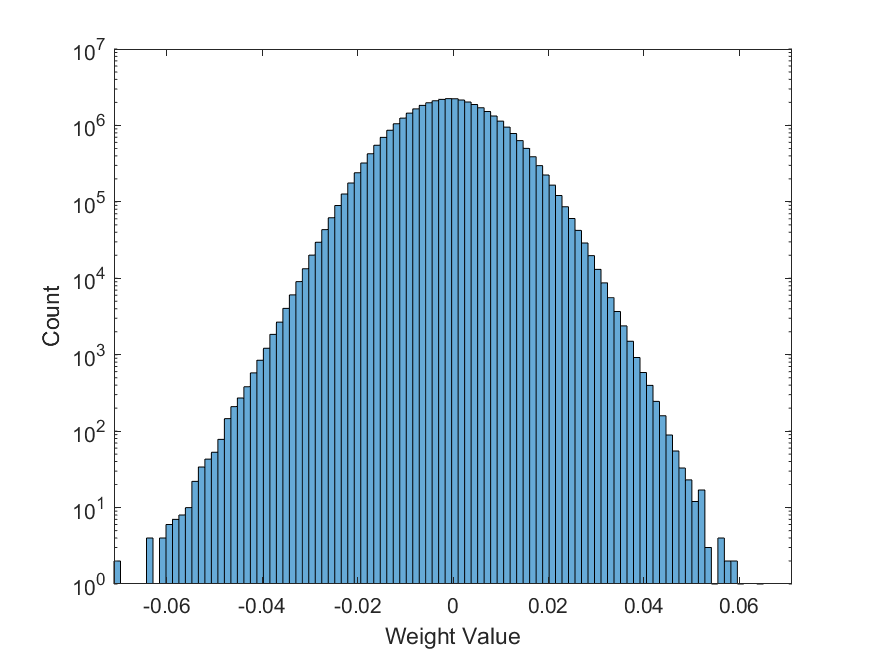
\includegraphics[scale=0.9]{Images/Weights/weight-distribution-FC1.png}
	\decoRule
	\caption[Weights distribution of 1st FC layer]{Weights distribution of 1st FC layer}
	\label{fig:weight-distribution-FC1}
\end{figure}

\begin{figure} [H]
	\centering
	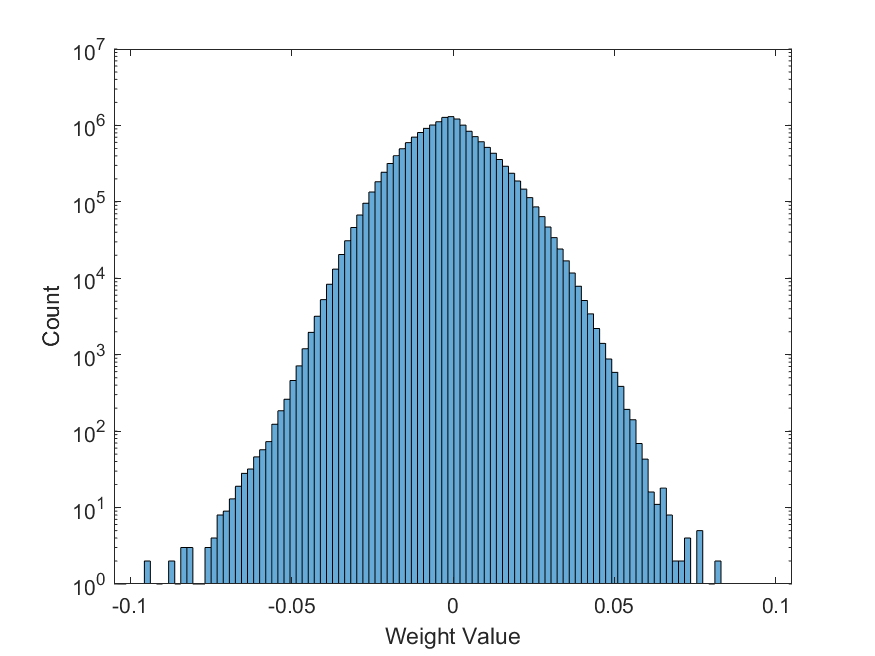
\includegraphics[scale=0.9]{Images/Weights/weight-distribution-FC2.png}
	\decoRule
	\caption[Weights distribution of 2nd FC layer]{Weights distribution of 2nd FC layer}
	\label{fig:weight-distribution-FC2}
\end{figure}

\begin{figure} [H]
	\centering
	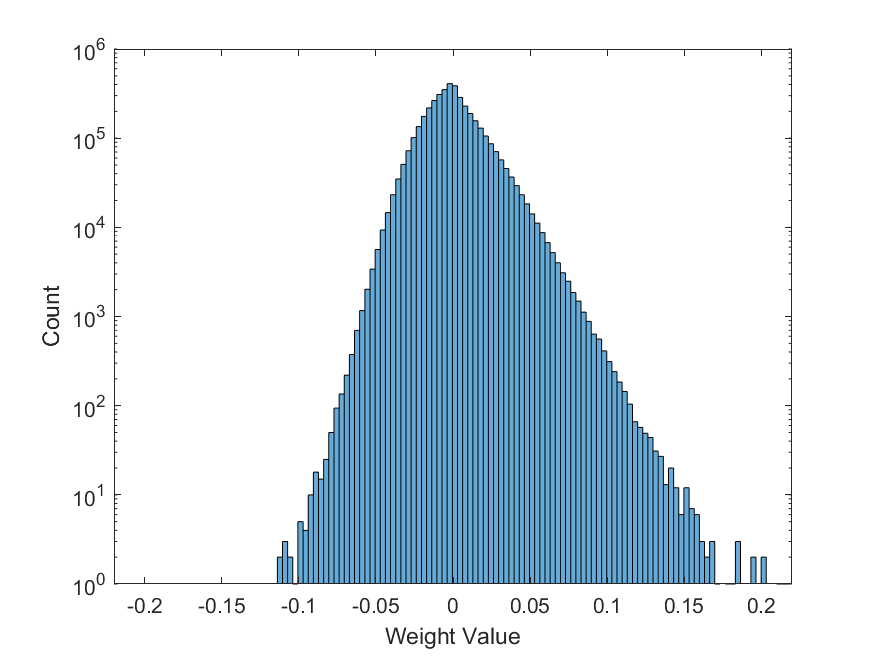
\includegraphics[scale=0.9]{Images/Weights/weight-distribution-FC3.png}
	\decoRule
	\caption[Weights distribution of 3rd FC layer]{Weights distribution of 3rd FC layer}
	\label{fig:weights-distribution-FC3}
\end{figure}
